% !TEX root = ../ms.tex

\defmath\B{\mathbb B}

\vspace{-1em}
\section{Introduction~\label{sec:introduction}}

%The simulation of quantum computing circuits is important for studying noise, synthesizing and optimizing circuits and 

Classical simulation of quantum computing is useful for circuit design~\cite{zulehner2017one} and studying noise resilience in the era of Noisy Intermediate-Scale Quantum (NISQ) computers~\cite{preskill2018quantum}.
Moreover, identifying classes of quantum circuits that are classically simulatable, helps in excluding regions where a quantum computational advantage cannot be obtained.
For example, circuits containing only Clifford gates (a non-universal quantum gate set), using an all-zero initial state, only compute the so-called `stabilizer states' and can be simulated in polynomial time
\cite{gottesman1998heisenberg,aaronson2008improved,gottesman1997stabilizer}.
%Stabilizer states arise when computing using only Clifford gates (a non-universal quantum gate set), and
Stabilizer states, and associated formalisms for expressing them, are fundamental to many quantum error correcting codes~\cite{gottesman1997stabilizer} and play a role in measurement-based quantum computation~\cite{raussendorf2001oneway}.
% circuit limited to the Clifford gate set stay in a tractable region of the so-called stabilizer states , which forms the basis for measurement-based quantum computation~\cite{raussendorf2001oneway} and many quantum error correction codes.
In fact, simulation of general quantum circuits is fixed-parameter tractable in the number of non-Clifford gates~\cite{bravyi2016trading}, a principle on which many modern simulators are based~\cite{bravyi2016trading,bravyi2017improved,bravyi2019simulation, huang2019approximate,kocia2018stationary,kocia2020improved}.

\begin{wrapfigure}{R}{.35\textwidth}\vspace{-1.5em}
	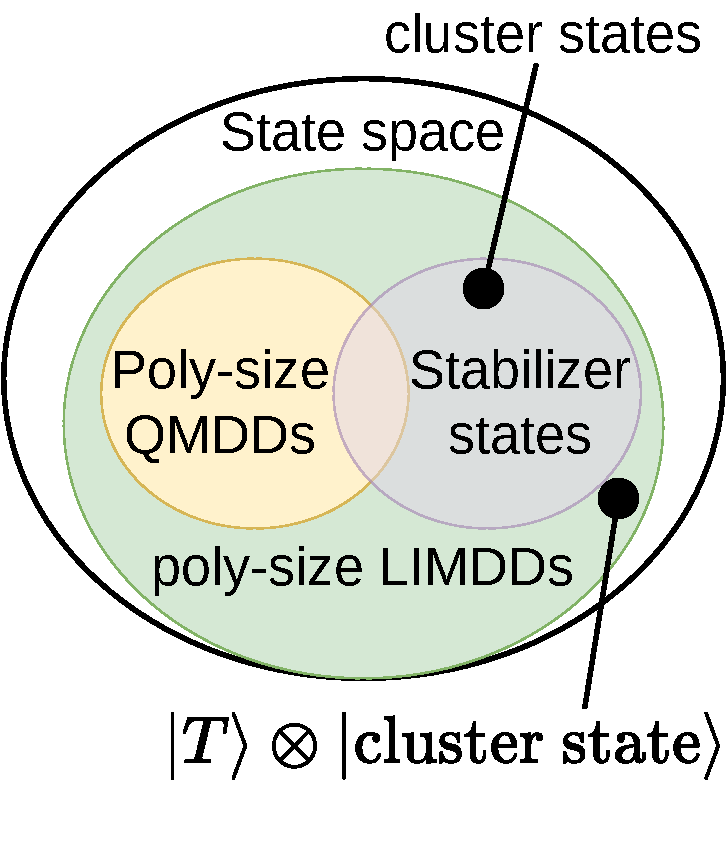
\includegraphics[width=.24\textwidth]{pics/venn-diagram.pdf}
    \centering
    \vspace{-1em}
	\caption{
        The set of stabilizer states and states represented as:
        poly-sized \limdds and QMDDs.
        \vspace{-\baselineskip}
	}%\vspace{-.5em}
    \label{fig:venn-diagram} 
\end{wrapfigure}

Another method for simulating universal quantum computation is based on (algebraic) decision diagrams (DDs)~\cite{akers1978binary,bryant86,580054,bryant1995verification,sanner,10.1145/157485.164569,fujita1997multi,viamontes2003improving,viamontes2004high,miller2006qmdd,zulehner2018advanced}.
A DD is a directed acyclic graph (DAG) in which each path represents a quantum amplitude, enabling the succinct representation of many quantum states through the combinatorial nature of these paths.
Various manipulation operations for DDs exist which implement any quantum gate operation in polynomial time
in the size of the DD. Together with other DD operations that can be used for measurement,
strong simulation is easily implemented using a DD data structure~\cite{miller2006qmdd,zulehner2018advanced}.
Indeed, DD-based simulation was empirically shown to be competitive with state-of-the-art simulators~\cite{viamontes2004high,zulehner2018advanced} and is used in several simulator implementations~\cite{viamontes2009quantum}.
%\todo{Vedran: at-the time? I mean, simulators have advanced a lot since 2018... As I mentioned they simulated shor on 60 qubits. good luck with that in any other method.}.
DDs and the stabilizer formalism are introduced in \autoref{sec:preliminaries}.
%However, in contrast to the stabilizer formalism, little is known about which quantum circuits are efficiently simulatable with DD-based approaches.


In this paper, we show that certain stabilizer states, called cluster states \cite{briegel2000persistent}, yield exponentially large \qmdds, the currently most succinct version of DDs
(see \autoref{sec:exponential-separations}).
In order to unite the strengths of DDs and the stabilizer formalism,
in \autoref{sec:isomorphism-qmdd}, we propose \limdd: a new DD for quantum computing simulation using local invertible maps (LIMs).
Specifically, \limdds eliminate the need to store multiple states which are equivalent up to LIMs, allowing more succinct DD representations.
%\todo{Tim: please check, it might sound a bit like \limdds only can encode stabilizer states now}
We prove that the set of quantum states that can be \emph{represented} by poly-sized \limdds 
is larger than those that can be expressed in either the stabilizer formalism or a poly-sized \qmdd.
\autoref{fig:venn-diagram} shows the resulting separation.
In \autoref{sec:quantum-simulation}, we give procedures for analyzing and simulating quantum 
circuits using \limdds and conclude in \autoref{sec:discussion} with evidence that \limdd-based simulation can be powerful than modern techniques using low-rank stabilizer decomposition~\cite{bravyi2019simulation}.

The workhorse behind \limdds is a novel algorithm which merges two DD nodes when they are `isomorphic:'
Two quantum states $\ket{\phi}$ and $\ket{\psi}$ are isomorphic when there is a series of Pauli operators $P_j$ and a complex nonzero number $\lambda$ such that $\ket{\phi}=\lambda P_n\otimes\cdots\otimes P_1\ket \psi$.
There is a plethora of work on investigating the effect of similar local operations in the context of stabilizer states \cite{nest2005local, englbrecht2020symmetries}; we emphasize that here we consider arbitrary quantum states $\ket{\phi}, \ket{\psi}$.%\todo{Tim: should rephrase, now it looks like no-one ever thought of considering locally-equivalent states beyond stabilizer states...}
To find such an isomorphism, we compute (generators of) the stabilizer (sub)group $\Stab(\ket \psi)$ of the state $\ket \psi$ represented by each DD node, and then we exploit the fact that the set of all such isomorphisms can be expressed as the coset $\pi\cdot \Stab(\ket \psi)$ for some isomorphism $\pi$.
To make the diagram canonical ---an important property for realizing efficient manipulation operations~\cite{darwiche2002knowledge}---
our algorithm then chooses a ``lexicographically smallest'' element from a Pauli coset.

%\todo[inline]{Vedran: general comment: i am a bit worried that nothing about efficiency of algorithms for all the manipulations is said for such a long time... I lose the connection to simulation of circuits... The Introduction for me is missing a link and clarification of the relationship between representation and simulation."}


%\todo[inline]{Give another / better example of polytime simulatable QC; introduce stabilizer states before they are mentioned.}

%\todo[inline]{Process Vedran's feedback, so write something about Clifford gates that's actually true.}

%This work is organized as follows.
%After providing the necessary background in \autoref{sec:preliminaries}, we formally introduce \limdds in \autoref{sec:isomorphism-qmdd}.
%In \autoref{sec:exponential-separations}, we prove the exponential separation between QMDDs and \limdds, by showing that there is a sequence of $n$-qubit stabilizer states that can only be represented with exponentially-sized QMDDs.






